% ============================================================
\chapter{Motivations --- G\'eom\'etrie en Deep Learning}
\label{ch:motivations}
% ============================================================

Les r\'eseaux de neurones classiques --- perceptrons, CNN, RNN --- sont
con\c{c}us pour des donn\'ees vivant sur des grilles r\'eguli\`eres~: images
sur des pixels, s\'eries temporelles sur des pas de temps uniform\'ement
espac\'es. Mais que faire quand les donn\'ees vivent sur un graphe (r\'eseaux
sociaux, mol\'ecules), sur une surface courbe (mod\`eles 3D), ou sur un
groupe de sym\'etries (poses, rotations)~? C'est la question \`a laquelle
r\'epond l'\emph{apprentissage g\'eom\'etrique}~: une r\'evolution
architecturale, port\'ee par les travaux de Bronstein, Bruna, Cohen, et
d'autres, qui replace la g\'eom\'etrie au c\oe ur du deep learning.

% ------------------------------------------------------------
\section{Les limites des architectures classiques}
% ------------------------------------------------------------

Les r\'eseaux de neurones convolutifs (CNN) ont connu un succ\`es spectaculaire
en vision par ordinateur, traitement du signal et reconnaissance vocale. Leur
puissance provient d'un \textbf{biais inductif} fondamental~: l'exploitation
de la structure de grille r\'eguli\`ere des donn\'ees.

\begin{definition}[Biais inductif]
Un \textbf{biais inductif} est un ensemble d'hypoth\`eses a priori incorpor\'ees
dans l'architecture d'un mod\`ele pour guider l'apprentissage. Pour un CNN~:
\begin{enumerate}
    \item \textbf{Localit\'e}~: chaque neurone ne regarde qu'un voisinage local.
    \item \textbf{Partage des poids}~: le m\^eme filtre est appliqu\'e partout.
    \item \textbf{Invariance par translation}~: la d\'etection de motifs est
          ind\'ependante de la position.
\end{enumerate}
\end{definition}

Cependant, de nombreuses donn\'ees du monde r\'eel n'ont \textbf{pas} de structure
de grille~:

\begin{exemple}[Donn\'ees non euclidiennes]
\begin{enumerate}
    \item Une \textbf{mol\'ecule} est un graphe d'atomes reli\'es par des liaisons chimiques.
    \item Un \textbf{r\'eseau social} est un graphe de personnes reli\'ees par des relations.
    \item La \textbf{surface de la Terre} est une sph\`ere, pas un plan.
    \item Un \textbf{nuage de points} 3D issu d'un capteur LiDAR n'a pas d'ordre canonique.
\end{enumerate}
\end{exemple}

\begin{attention}[title=\textbf{Pourquoi ne pas simplement vectoriser~?}]
On pourrait \^etre tent\'e de repr\'esenter un graphe par sa matrice d'adjacence
aplatie en vecteur et d'utiliser un MLP. Cette approche \'echoue car~:
\begin{itemize}
    \item La repr\'esentation d\'epend de la \textbf{num\'erotation arbitraire} des n\oe uds.
    \item Le nombre de param\`etres explose~: $\mathcal{O}(n^2)$ pour $n$ n\oe uds.
    \item Aucune \textbf{g\'en\'eralisation} \`a des graphes de tailles diff\'erentes.
\end{itemize}
\end{attention}

\section{La g\'eom\'etrie comme principe organisateur}

\subsection{Le programme d'Erlangen}

En 1872, Felix Klein proposa dans son \textit{Erlanger Programm} de classifier
les g\'eom\'etries par leurs groupes de sym\'etries. Cette id\'ee profonde trouve
une application directe en apprentissage profond.

\begin{theoreme}[Programme d'Erlangen --- version informelle]
Une g\'eom\'etrie est enti\`erement d\'etermin\'ee par son \textbf{groupe de
transformations} $G$ et les propri\'et\'es qui sont \textbf{invariantes} sous
l'action de $G$.
\end{theoreme}

\begin{exemple}[G\'eom\'etries et leurs groupes]
\begin{center}
\begin{tabular}{lll}
\toprule
\textbf{G\'eom\'etrie} & \textbf{Groupe} & \textbf{Invariants} \\
\midrule
Euclidienne & Isom\'etries $\mathrm{E}(n)$ & Distances, angles \\
Affine & Transformations affines & Parall\'elisme, rapports \\
Projective & Transformations projectives & Rapport biharmonique \\
\bottomrule
\end{tabular}
\end{center}
\end{exemple}

\subsection{Des CNN aux GNN~: le passage de la grille au graphe}

Un CNN peut \^etre vu comme un cas particulier de r\'eseau op\'erant sur un
graphe r\'egulier (la grille de pixels), avec le groupe de translation
$\Z^2$ comme groupe de sym\'etries.

\begin{formules}[title=\textbf{Convolution discr\`ete sur grille vs.\ graphe}]
\textbf{Convolution sur grille}~:
\[
    (f * g)(x) = \sum_{y \in \Z^2} f(y)\, g(x - y)
\]
\textbf{Convolution sur graphe} (passage de messages)~:
\[
    \mathbf{h}_v^{(\ell+1)} = \phi\!\left(\mathbf{h}_v^{(\ell)},\;
    \bigoplus_{u \in \mathcal{N}(v)} \psi\!\left(\mathbf{h}_v^{(\ell)},
    \mathbf{h}_u^{(\ell)}, \mathbf{e}_{uv}\right)\right)
\]
\end{formules}

\begin{figure}[htbp]
\centering
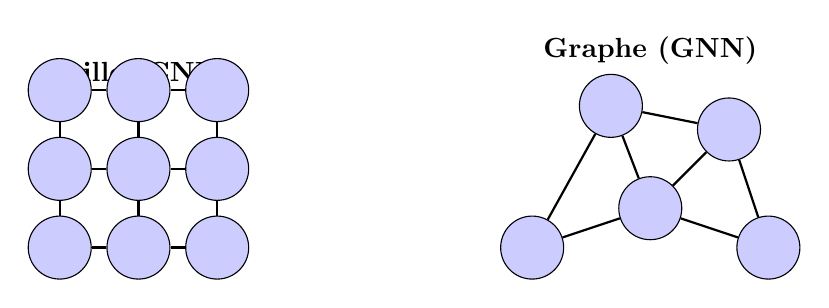
\begin{tikzpicture}[
    node_style/.style={circle, draw, fill=blue!20, minimum size=8mm, inner sep=0pt},
    edge_style/.style={thick, -}
]
% Grille 3x3
\begin{scope}[shift={(-4,0)}]
    \node[font=\bfseries] at (1, 2.2) {Grille (CNN)};
    \foreach \i in {0,1,2} {
        \foreach \j in {0,1,2} {
            \node[node_style] (g\i\j) at (\i, \j) {};
        }
    }
    \foreach \i in {0,1,2} {
        \foreach \j [evaluate=\j as \jn using int(\j+1)] in {0,1} {
            \draw[edge_style] (g\i\j) -- (g\i\jn);
        }
    }
    \foreach \j in {0,1,2} {
        \foreach \i [evaluate=\i as \in using int(\i+1)] in {0,1} {
            \draw[edge_style] (g\i\j) -- (g\in\j);
        }
    }
\end{scope}
% Graphe irregulier
\begin{scope}[shift={(2,0)}]
    \node[font=\bfseries] at (1.5, 2.5) {Graphe (GNN)};
    \node[node_style] (a) at (0, 0) {};
    \node[node_style] (b) at (1, 1.8) {};
    \node[node_style] (c) at (2.5, 1.5) {};
    \node[node_style] (d) at (3, 0) {};
    \node[node_style] (e) at (1.5, 0.5) {};
    \draw[edge_style] (a) -- (b);
    \draw[edge_style] (b) -- (c);
    \draw[edge_style] (c) -- (d);
    \draw[edge_style] (a) -- (e);
    \draw[edge_style] (e) -- (b);
    \draw[edge_style] (e) -- (c);
    \draw[edge_style] (e) -- (d);
\end{scope}
\end{tikzpicture}
\caption{Passage d'une grille r\'eguli\`ere (CNN) \`a un graphe irr\'egulier (GNN).}
\label{fig:grid_vs_graph}
\end{figure}

\section{Le cadre unificateur~: Geometric Deep Learning}

\subsection{Les cinq G}

Bronstein et al.\ (2021) ont propos\'e un cadre unificateur organis\'e autour
de cinq domaines fondamentaux~:

\begin{definition}[Domaines du GDL]
\begin{enumerate}
    \item \textbf{Grilles} ($\Omega = \Z^d$)~: sym\'etrie de translation.
    \item \textbf{Groupes} ($\Omega = G$)~: sym\'etrie par le groupe lui-m\^eme.
    \item \textbf{Graphes} ($\Omega = (V,E)$)~: sym\'etrie par permutation $S_n$.
    \item \textbf{G\'eod\'esiques} ($\Omega = \mathcal{M}$)~: invariance par isom\'etries.
    \item \textbf{Jauges} ($\Omega = \mathcal{M}$ avec fibr\'e)~: \'equivariance de jauge.
\end{enumerate}
\end{definition}

\subsection{Le principe g\'en\'eral d'\'equivariance}

\begin{theoreme}[Principe d'\'equivariance]
Soit $\mathfrak{G}$ un groupe agissant sur un espace de signaux
$\mathcal{X}(\Omega)$ via la repr\'esentation $\rho_{\mathcal{X}}$ et sur un
espace cible $\mathcal{Y}$ via $\rho_{\mathcal{Y}}$. Une fonction
$f: \mathcal{X}(\Omega) \to \mathcal{Y}$ est \textbf{\'equivariante} si~:
\[
    f\bigl(\rho_{\mathcal{X}}(g) \cdot x\bigr) = \rho_{\mathcal{Y}}(g) \cdot f(x),
    \quad \forall g \in \mathfrak{G},\; \forall x \in \mathcal{X}(\Omega).
\]
Lorsque $\rho_{\mathcal{Y}}$ est la repr\'esentation triviale, $f$ est
\textbf{invariante}.
\end{theoreme}

\begin{intuition}[title=\textbf{\'Equivariance en images}]
Consid\'erons la classification d'images~:
\begin{itemize}
    \item Les couches convolutives sont \textbf{\'equivariantes} par translation~:
          si l'entr\'ee se d\'eplace, les cartes d'activation se d\'eplacent aussi.
    \item Le pooling global produit une sortie \textbf{invariante}~: le r\'esultat
          ne d\'epend pas de la position de l'objet.
\end{itemize}
Le m\^eme principe s'applique aux GNN~: les couches de passage de messages sont
\'equivariantes par permutation des n\oe uds, et le readout global est invariant.
\end{intuition}

\section{L'importance de l'invariance par permutation}

\subsection{Formalisation}

Pour un graphe \`a $n$ n\oe uds, une \textbf{permutation} $\pi \in S_n$ r\'eordonne
les n\oe uds. Cela agit sur~:
\begin{itemize}
    \item La matrice d'adjacence~: $\mathbf{A} \mapsto \mathbf{P}_\pi \mathbf{A} \mathbf{P}_\pi^\top$
    \item Les attributs~: $\mathbf{X} \mapsto \mathbf{P}_\pi \mathbf{X}$
\end{itemize}
o\`u $\mathbf{P}_\pi$ est la matrice de permutation associ\'ee \`a $\pi$.

\begin{definition}[Fonction invariante / \'equivariante sur graphes]
Une fonction au niveau du graphe $f: (\mathbf{A}, \mathbf{X}) \mapsto y$
est \textbf{invariante par permutation} si~:
\[
    f(\mathbf{P}_\pi \mathbf{A} \mathbf{P}_\pi^\top, \mathbf{P}_\pi \mathbf{X})
    = f(\mathbf{A}, \mathbf{X}), \quad \forall \pi \in S_n.
\]
Une fonction au niveau des n\oe uds $f: (\mathbf{A}, \mathbf{X}) \mapsto \mathbf{H}$
est \textbf{\'equivariante par permutation} si~:
\[
    f(\mathbf{P}_\pi \mathbf{A} \mathbf{P}_\pi^\top, \mathbf{P}_\pi \mathbf{X})
    = \mathbf{P}_\pi f(\mathbf{A}, \mathbf{X}), \quad \forall \pi \in S_n.
\]
\end{definition}

\subsection{Deep Sets~: le cas le plus simple}

\begin{theoreme}[Zaheer et al., 2017]
Une fonction $f: 2^{\mathcal{X}} \to \R$ est invariante par permutation et
continue si et seulement si elle peut s'\'ecrire sous la forme~:
\[
    f(\{x_1, \ldots, x_n\}) = \rho\!\left(\sum_{i=1}^{n} \phi(x_i)\right)
\]
pour des fonctions continues $\phi: \mathcal{X} \to \R^d$ et
$\rho: \R^d \to \R$.
\end{theoreme}

\begin{codeblock}[title=\textbf{Impl\'ementation Deep Sets en PyTorch}]
\begin{minted}{python}
import torch
import torch.nn as nn

class DeepSets(nn.Module):
    """Modele invariant par permutation pour ensembles."""
    def __init__(self, input_dim, hidden_dim, output_dim):
        super().__init__()
        # phi : encodeur par element
        self.phi = nn.Sequential(
            nn.Linear(input_dim, hidden_dim),
            nn.ReLU(),
            nn.Linear(hidden_dim, hidden_dim),
        )
        # rho : decodeur apres aggregation
        self.rho = nn.Sequential(
            nn.Linear(hidden_dim, hidden_dim),
            nn.ReLU(),
            nn.Linear(hidden_dim, output_dim),
        )

    def forward(self, x):
        # x: (batch, n_elements, input_dim)
        h = self.phi(x)           # (batch, n_elements, hidden_dim)
        h = h.sum(dim=1)          # (batch, hidden_dim) -- aggregation
        return self.rho(h)        # (batch, output_dim)

# Test
model = DeepSets(input_dim=3, hidden_dim=64, output_dim=10)
x = torch.randn(8, 20, 3)  # batch=8, 20 points, dim=3
out = model(x)
print(f"Sortie: {out.shape}")  # (8, 10)

# Verification de l'invariance par permutation
perm = torch.randperm(20)
x_perm = x[:, perm, :]
out_perm = model(x_perm)
print(f"Invariance: {torch.allclose(out, out_perm, atol=1e-5)}")
\end{minted}
\end{codeblock}

\section{Exemples motivants}

\subsection{Pr\'ediction de propri\'et\'es mol\'eculaires}

La pr\'ediction de propri\'et\'es mol\'eculaires est l'une des applications phares
du GDL. Une mol\'ecule est naturellement repr\'esent\'ee comme un graphe~:
\begin{itemize}
    \item \textbf{N\oe uds}~: atomes, avec attributs (type atomique, charge, etc.).
    \item \textbf{Ar\^etes}~: liaisons chimiques, avec attributs (ordre de liaison, etc.).
\end{itemize}

\begin{proposition}[Propri\'et\'es souhait\'ees]
Un mod\`ele pour la pr\'ediction mol\'eculaire doit \^etre~:
\begin{enumerate}
    \item \textbf{Invariant par permutation} des atomes (pas de num\'erotation canonique).
    \item \textbf{Invariant par rotation et translation} (\'energie ind\'ependante
          de l'orientation).
    \item \textbf{Extensif / intensif} selon la propri\'et\'e (\'energie vs.\ gap HOMO-LUMO).
\end{enumerate}
\end{proposition}

\subsection{M\'et\'eorologie sur la sph\`ere}

Les donn\'ees m\'et\'eorologiques vivent naturellement sur la sph\`ere $S^2$.
Les CNN classiques ne peuvent pas \^etre directement appliqu\'es car~:
\begin{itemize}
    \item Les projections planes introduisent des \textbf{distorsions} (Mercator, etc.).
    \item La grille de pixels n'est pas uniforme sur la sph\`ere.
    \item Les sym\'etries physiques (rotations) ne sont pas respect\'ees.
\end{itemize}

\begin{remarque}[Spherical CNNs]
Les \textit{Spherical CNNs} (Cohen et al., 2018) d\'efinissent des convolutions
directement sur $S^2$ en utilisant les harmoniques sph\'eriques comme base spectrale,
respectant ainsi l'\'equivariance par $\mathrm{SO}(3)$.
\end{remarque}

\subsection{Dynamique des particules}

La simulation de syst\`emes de particules (fluides, mat\'eriaux granulaires)
b\'en\'eficie du GDL car~:
\begin{itemize}
    \item Les particules forment un ensemble non ordonn\'e.
    \item Les lois physiques sont \'equivariantes par $\mathrm{SE}(3)$.
    \item Les interactions sont locales (graphe de voisinage).
\end{itemize}

\section{Panorama des architectures g\'eom\'etriques}

\begin{figure}[htbp]
\centering
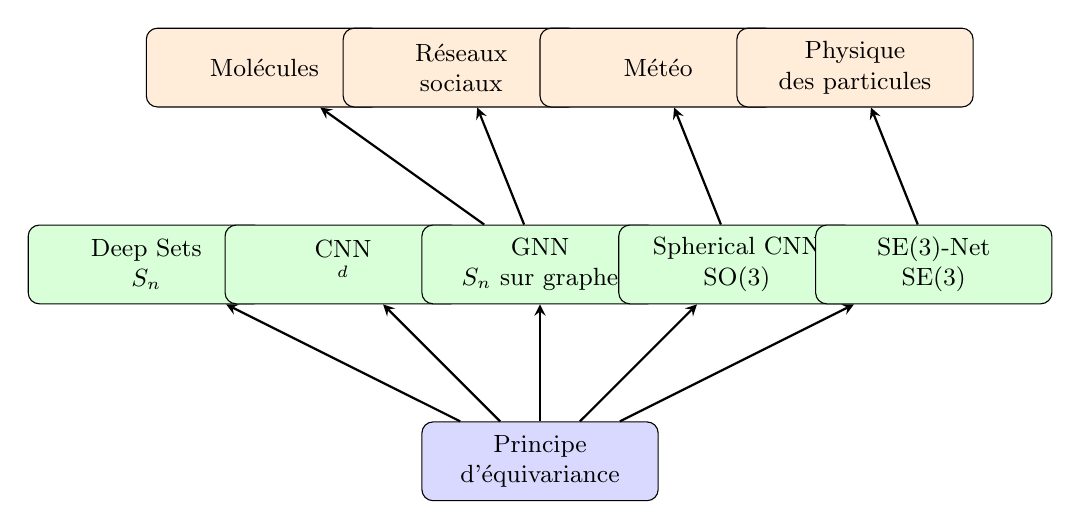
\begin{tikzpicture}[
    box/.style={rectangle, draw, rounded corners, fill=#1!15,
                minimum width=3cm, minimum height=1cm, align=center,
                font=\small},
    arr/.style={->, thick, >=stealth}
]
\node[box=blue] (base) at (0, 0) {Principe\\d'\'equivariance};
\node[box=green] (ds) at (-5, 2.5) {Deep Sets\\$S_n$};
\node[box=green] (cnn) at (-2.5, 2.5) {CNN\\$\Z^d$};
\node[box=green] (gnn) at (0, 2.5) {GNN\\$S_n$ sur graphe};
\node[box=green] (scnn) at (2.5, 2.5) {Spherical CNN\\$\mathrm{SO}(3)$};
\node[box=green] (se3) at (5, 2.5) {SE(3)-Net\\$\mathrm{SE}(3)$};

\draw[arr] (base) -- (ds);
\draw[arr] (base) -- (cnn);
\draw[arr] (base) -- (gnn);
\draw[arr] (base) -- (scnn);
\draw[arr] (base) -- (se3);

\node[box=orange] (mol) at (-3.5, 5) {Mol\'ecules};
\node[box=orange] (soc) at (-1, 5) {R\'eseaux\\sociaux};
\node[box=orange] (met) at (1.5, 5) {M\'et\'eo};
\node[box=orange] (phys) at (4, 5) {Physique\\des particules};

\draw[arr] (gnn) -- (mol);
\draw[arr] (gnn) -- (soc);
\draw[arr] (scnn) -- (met);
\draw[arr] (se3) -- (phys);
\end{tikzpicture}
\caption{Panorama des architectures g\'eom\'etriques et de leurs applications.}
\end{figure}

\section{Pourquoi les sym\'etries am\'eliorent l'apprentissage}

L'exploitation des sym\'etries am\'eliore l'apprentissage de trois mani\`eres
compl\'ementaires~:

\begin{theoreme}[Avantages de l'\'equivariance]
Soit $\mathfrak{G}$ le groupe de sym\'etries d'un probl\`eme. Un mod\`ele
\'equivariant par $\mathfrak{G}$ b\'en\'eficie de~:
\begin{enumerate}
    \item \textbf{R\'eduction de la complexit\'e d'\'echantillonnage}~: le nombre
          d'exemples n\'ecessaires est r\'eduit d'un facteur $\abs{\mathfrak{G}}$
          (ou de la dimension du groupe pour les groupes continus).
    \item \textbf{Am\'elioration de la g\'en\'eralisation}~: la garantie de
          g\'en\'eralisation \`a toutes les transformations de $\mathfrak{G}$
          est \og gratuite \fg.
    \item \textbf{Partage des poids}~: le nombre de param\`etres est r\'eduit,
          \'evitant le surapprentissage.
\end{enumerate}
\end{theoreme}

\begin{proposition}[Borne de g\'en\'eralisation]
Pour un mod\`ele param\'etr\'e par $\theta \in \Theta$, la complexit\'e de Rademacher
de la classe de fonctions \'equivariantes $\mathcal{F}_{\text{equiv}}$ satisfait~:
\[
    \mathfrak{R}_n(\mathcal{F}_{\text{equiv}}) \leq
    \frac{\mathfrak{R}_n(\mathcal{F})}{\sqrt{\abs{\mathfrak{G}}}}
\]
o\`u $\mathcal{F}$ est la classe non contrainte.
\end{proposition}

\section{De la th\'eorie \`a la pratique}

\begin{codeblock}[title=\textbf{Premier GNN avec PyTorch Geometric}]
\begin{minted}{python}
import torch
import torch.nn.functional as F
from torch_geometric.nn import GCNConv, global_mean_pool
from torch_geometric.datasets import TUDataset
from torch_geometric.loader import DataLoader

class SimpleGNN(torch.nn.Module):
    def __init__(self, num_features, num_classes):
        super().__init__()
        self.conv1 = GCNConv(num_features, 64)
        self.conv2 = GCNConv(64, 64)
        self.lin = torch.nn.Linear(64, num_classes)

    def forward(self, data):
        x, edge_index, batch = data.x, data.edge_index, data.batch
        # Couches equivariantes par permutation
        x = F.relu(self.conv1(x, edge_index))
        x = F.relu(self.conv2(x, edge_index))
        # Readout invariant par permutation
        x = global_mean_pool(x, batch)
        return self.lin(x)

# Charger un dataset de classification de graphes
dataset = TUDataset(root='/tmp/MUTAG', name='MUTAG')
loader = DataLoader(dataset, batch_size=32, shuffle=True)

model = SimpleGNN(dataset.num_features, dataset.num_classes)
optimizer = torch.optim.Adam(model.parameters(), lr=0.01)

# Boucle d'entrainement
for epoch in range(50):
    total_loss = 0
    for data in loader:
        optimizer.zero_grad()
        out = model(data)
        loss = F.cross_entropy(out, data.y)
        loss.backward()
        optimizer.step()
        total_loss += loss.item()
    if (epoch + 1) % 10 == 0:
        print(f"Epoch {epoch+1}, Loss: {total_loss/len(loader):.4f}")
\end{minted}
\end{codeblock}

\section{Plan du cours et d\'ependances}

\begin{figure}[htbp]
\centering
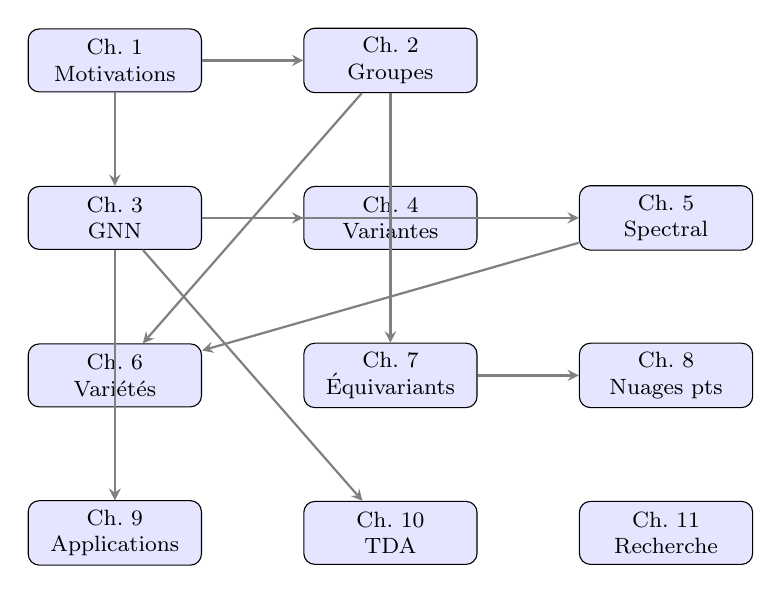
\begin{tikzpicture}[
    ch/.style={rectangle, draw, rounded corners, fill=blue!10,
               minimum width=2.2cm, minimum height=0.8cm,
               align=center, font=\footnotesize},
    dep/.style={->, thick, >=stealth, gray}
]
\node[ch] (c1) at (0, 0) {Ch.~1\\Motivations};
\node[ch] (c2) at (3.5, 0) {Ch.~2\\Groupes};
\node[ch] (c3) at (0, -2) {Ch.~3\\GNN};
\node[ch] (c4) at (3.5, -2) {Ch.~4\\Variantes};
\node[ch] (c5) at (7, -2) {Ch.~5\\Spectral};
\node[ch] (c6) at (0, -4) {Ch.~6\\Vari\'et\'es};
\node[ch] (c7) at (3.5, -4) {Ch.~7\\\'Equivariants};
\node[ch] (c8) at (7, -4) {Ch.~8\\Nuages pts};
\node[ch] (c9) at (0, -6) {Ch.~9\\Applications};
\node[ch] (c10) at (3.5, -6) {Ch.~10\\TDA};
\node[ch] (c11) at (7, -6) {Ch.~11\\Recherche};

\draw[dep] (c1) -- (c2);
\draw[dep] (c1) -- (c3);
\draw[dep] (c2) -- (c7);
\draw[dep] (c3) -- (c4);
\draw[dep] (c3) -- (c5);
\draw[dep] (c2) -- (c6);
\draw[dep] (c5) -- (c6);
\draw[dep] (c7) -- (c8);
\draw[dep] (c3) -- (c9);
\draw[dep] (c6) -- (c9);
\draw[dep] (c3) -- (c10);
\end{tikzpicture}
\caption{Graphe de d\'ependances entre les chapitres.}
\end{figure}

\section*{Exercices}

\begin{exercice}[Invariance vs.\ \'equivariance]
Soit $f: \R^{n \times d} \to \R^{n \times d'}$ d\'efinie par
$f(\mathbf{X}) = \sigma(\mathbf{X}\mathbf{W})$ o\`u $\mathbf{W} \in \R^{d \times d'}$.
\begin{enumerate}
    \item Montrer que $f$ est \'equivariante par permutation des lignes de $\mathbf{X}$.
    \item Proposer une modification de $f$ pour obtenir une fonction invariante
          $g: \R^{n \times d} \to \R^{d'}$.
    \item Impl\'ementer les deux fonctions en PyTorch et v\'erifier exp\'erimentalement.
\end{enumerate}
\end{exercice}

\begin{exercice}[Limites de la vectorisation]
Consid\'erons un graphe al\'eatoire $G \sim \mathrm{Erd\H{o}s\text{-}R\'enyi}(n, p)$.
\begin{enumerate}
    \item Combien de repr\'esentations matricielles diff\'erentes $\mathbf{A}$
          correspondent au m\^eme graphe (isomorphe)~?
    \item En d\'eduire pourquoi un MLP appliqu\'e \`a $\mathrm{vec}(\mathbf{A})$ a
          une complexit\'e d'\'echantillonnage exponentielle.
    \item Montrer qu'un GNN \'evite ce probl\`eme par construction.
\end{enumerate}
\end{exercice}

\begin{exercice}[Deep Sets pour l'approximation de fonctions sym\'etriques]
Impl\'ementer un mod\`ele Deep Sets pour approximer la fonction
$f(\{x_1, \ldots, x_n\}) = \max_i x_i - \min_i x_i$ (l'\'etendue d'un ensemble).
\begin{enumerate}
    \item Entra\^iner le mod\`ele sur des ensembles de taille variable $n \in [5, 50]$.
    \item \'Evaluer la g\'en\'eralisation \`a $n = 100$.
    \item Comparer avec une agr\'egation par $\max$ au lieu de la somme.
\end{enumerate}
\end{exercice}
